\documentclass[twocolumn]{revtex4}
\usepackage[]{graphicx}

\begin{document}

\title{
Is it Possible to Escape a Velociraptor?
}

\author{Ryan Mikulec}
\affiliation{Siena College, Loudonville, NY}
\date{\today}

\begin{abstract}
    Due to the underdevelopment in today's Jurassic cloning technology, we are unable to obtain  an 
    actual velociraptor to find out if us, humans, are able to escape one in an encounter.
    The next best thing is to run a computer simulation to test this
    unusual situation. The simulation is broken down into 4 parts, with a few assumptions.
    The first part is graphing the positions of the two subject. The second is finding out 
    where and when the raptor will catch up. The third is where an how far will the raptor 
    and human have traveled when they are one meter apart. The final part involves finding
    the probability that a human will escape this dangerous encounter. For the entirety of the
    code we will be assuming that the raptor and the human both accelerate instantaneously. Upon
    running the code it was found that it would take around 2 seconds for the velociraptor to 
    travel 6 meters to catch up to the human, assuming the human got a 30 meter head start. At
    around 1.94 seconds the raptor would have travel almost 35 meters, placing it 1 meter behind
    the human. When it is 1 meter behind, it was found, using a Monte Carlo simulation, that 
    there would be a 63 percent chance of escaping.
\end{abstract}

\maketitle
%%%%%%%%%%%%%%%%%%%%%%%%%%%%%%%%%%%%%%%%%%%%%%%%%%%%%%%%%%%%%%%%%%%%%%%%%%%%%%%%

%%%%%%%%%%%%%%%%%%%%%%%%%%%%%%%%%%%%%%%%%%%%%%%%%%%%%%%%%%%%%%%%%%%%%%%%%%%%%%%%
\section{Graphing the positions}
%%%%%%%%%%%%%%%%%%%%%%%%%%%%%%%%%%%%%%%%%%%%%%%%%%%%%%%%%%%%%%%%%%%%%%%%%%%%%%%%
	The purpose of this section was to display a position versus time graph
	containing both the velociraptor and the human. Below is the code that was used.\\
\begin{figure}[h!]
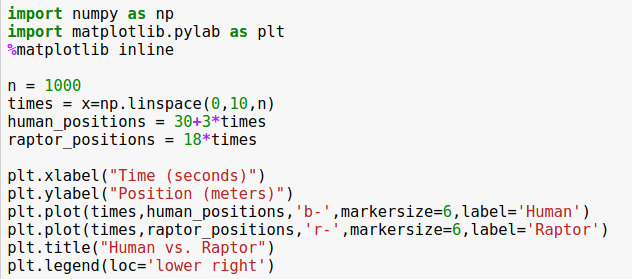
\includegraphics[width=0.5\textwidth]{Code1.png}
Code Section 1: This is the code used to obtain the graphs.
\end{figure}
	\\In order the graph the position, the first part was to derive an equation 
	for both the raptor and the human. By starting with the distance kinematics equation:
	$$x_1 = x_0 + v_0t + \frac{1}{2}at^2$$ 
	Because we are assuming they accelerating to their max velocities instantaneously
	acceleration is equal to 0, and by plugging in their velocities and starting positions, 
	the two linear equations come out to be:
	$$Raptor Postition = (18 \frac{m}{s})*t$$
	$$Human Position = 30m+(3 \frac{m}{s})*t$$
	\\
	\\
	\\
	\\In order to graph this, there has to be a corresponding set of time values
	to plug into these equations. That is what the function linspace is for. Linspace,
	imported from numpy, is used to create
	a list numbers with a given number of evenly spaced intervals between two numbers.
	In this case, a list called times was created, consisting of numbers between zero and
	ten, with n number of points. By using the times in the equations for positions, both
	human\_positions and raptor\_positions become lists that is then used in the plot function,
	imported on the top, to graph the values. The rest of the lines of code use functions part of
	plot to add a title, labels, and a legend. Below is the graph that was produced
\begin{figure}[h!]
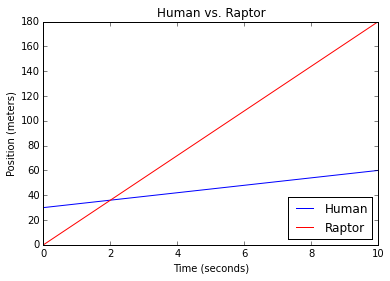
\includegraphics[width=0.5\textwidth]{Figure1.png}
Figure 1: Graph of the Human and Raptor positions

\end{figure}
\\
\\
\\
\\
\\

%%%%%%%%%%%%%%%%%%%%%%%%%%%%%%%%%%%%%%%%%%%%%%%%%%%%%%%%%%%%%%%%%%%%%%%%%%%%%%%%
\section{Finding where they meet}
	The purpose of the section is to use the results from part 1, to determine where and the the 	raptor and human will be at the same position. Below is the code that was used to
	do so.\\
\begin{figure}[h!]
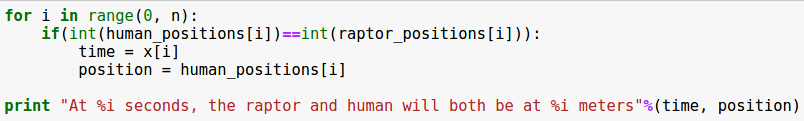
\includegraphics[width=0.5\textwidth]{Code2.png}
Code Section 2: Used to determine equal position and time

\end{figure}
\\The main feature of this code is the for statement. This for statement runs n+1 amount of times, each time changing the integer i to the corresponding value of the trial its on. It is set to n, because n was used in part 1 to determine the number of values in the lists. By using this, the for statement is running to the number of values in the lists from part 1. Inside the for loop is an if statement that is checking to see if the value of human\_positions at i is equal to the value of raptor\_positions at i. If they are equal, it will continue to set a new variable called position to the value in human\_position, and set another new variable called time to the value in the times list at i. In summary, this loop runs through all the values in the human positions list, and the corresponding values in the raptor positions list, checking to see if they are equal, then recording them if they are. The values of the positions were turned into integers because due to linspace, there may not have existed a value in which this statement is true. By forcing them to be integers, it guaranteed that there is. It was found that after 2 seconds, both the positions are 36 meters.
%%%%%%%%%%%%%%%%%%%%%%%%%%%%%%%%%%%%%%%%%%%%%%%%%%%%%%%%%%%%%%%%%%%%%%%%%%%%%%%%

\section{1 meter away}
	The purpose of this section is to find when, and how far the raptor and human are 
	when they are one meter apart, then graphing these two points.Below is the code that was 	 used:
	\\
	\\

\begin{figure}[h!]
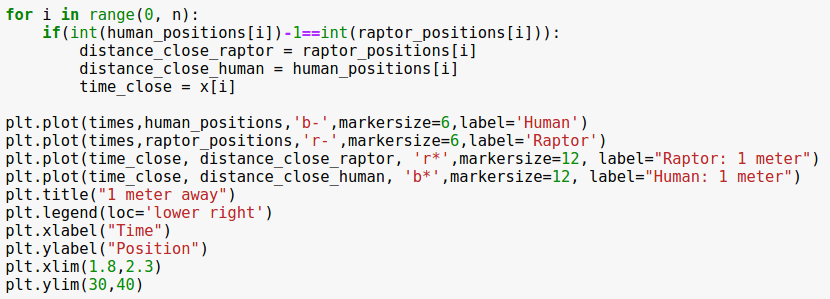
\includegraphics[width=0.5\textwidth]{Code3.png}
Code Section 3: Used to find distance 1 meter away 

\end{figure} 	
\section*{}
 A very similar approach
	to part 2 was used to accomplish this with one key difference. Instead of the if statement
	checking to see if they are equal, it is checking the see where the human position minus 
	the raptor position is equal to one. This was found with the process below:
	$$Raptor Position + 1 = Human Position$$
	$$Human Position - Raptor Position = 1$$
	These new values where then stored in the new variables, distance\_close\_raptor,
	distance\_close\_human, and time\_close. The final part was to produce the graph. The 
	imported plot function was used once again to create a graph very similar to that in
	part 1. Then the plot function was used again to plot the points that were obtained using
	the new close variables. The final step was adjusting the limits in order to show the
	relationship better. After around 1.94 seconds, the raptor travels around 34.8 meters, and the human travels around 5.8 meters from its initial 30, making them 1 meter apart. Below is the graph that was produced:
	
\begin{figure}[h!]
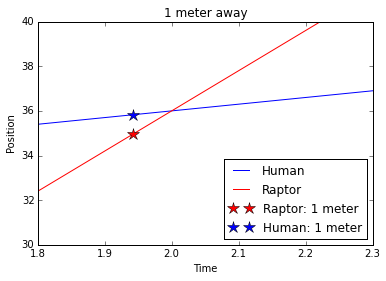
\includegraphics[width=0.5\textwidth]{Figure3.png}
Figure 2: Graph of the Human and Raptor positions when 1 meter apart

\end{figure} 

\section{What are the chances?}
	The purpose of this final section is to carry out a basic simulation to determine 
	a probability given a few assumptions.
	The first time the raptor tries to bite, there is a 20\% chance it will bite you. If it misses and tries a second time, there is only a 15\% chance, and if it misses that time, 			there is only a 7\% chance on the third try. The last assumption, based on common raptor
	behavior, is that if it misses that it will give up, and you will escape.
	\clearpage
The code below uses a Monte Carlo process to find the probability:
\begin{figure}[h!]
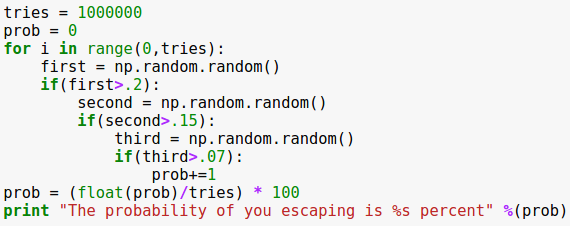
\includegraphics[width=0.5\textwidth]{Code4.png}
Code Section 4: Monte Carlo simulation

\end{figure} 
The purpose of a Monte Carlo simulation is to create a large amount of random numbers in order 
to obtain a simulated probability. This is done using three nested if statements inside a for loop that is executed an amount of times equal to the variable tries. Before the loop is a variable called prob then is set to be equal to 0, this is the counter. The first statement inside the for loop generates a random float between 0 and 1. The first if statement sees if this float is greater than the probability of the raptor biting you on its first try, which is .20. If it is greater then it continues to generate another random number and runs it through the second if statement, which sees if its greater than the second probability, which is .15. If this is true then it generates on last random number, throws it through a third if statement that sees if its greater than the third probability, which is .07. If this last statement is true then it will add one to the variable prob. By repeating this a tries number of times you are left with a ratio between prob, the number of times the third if statement was true, and tries, the number of times the loop was carried out. This ratio is the probability, and by multiplying it by 100, a percentage is obtained. The chance of you escaping based on this simulation came out to be around 63 \%. 
\\
\\
\\
\\
\\
\\
\\
\\
\\
\\
\\
\\
\\
\\
\\
\\
\\
\\
\\
\\
\\
\\
\\
\\
\\
\\
\\
\\
\\
\\
\\
\\
\\
\\
\\
\\
\\
\\
\\
\\
\\
\\
\\
\\
\\
\\
\\
\\
\\
\\
\\
\\
\\
\\
%%%%%%%%%%%%%%%%%%%%%%%%%%%%%%%%%%%%%%%%%%%%%%%%%%%%%%%%%%%%%%%%%%%%%%%%%%%%%%%%
\end{document}
%%%%%%%%%%%%%%%%%%%%%%%%%%%%%%%%%%%%%%%%%%%%%%%%%%%%%%%%%%%%%%%%%%%%%%%%%%%%%%%%
